% Cyber-Physical Control Systems 21/22
% Faculdade de Ciências e Tecnologia
% Universidade Nova de Lisboa
%
%	Project paper template
%
%	Author: Bruno Guerreiro, bj.guerreiro@fct.utl.pt, 2021
%
\documentclass[a4paper,twocolumn]{article}

% include packages
\usepackage{etex}
%\usepackage[portuguese]{babel} % if portuguese is the report language
\usepackage[utf8]{inputenc}
\usepackage{graphicx}
\usepackage{natbib}
\usepackage{epstopdf}
\usepackage{fancyhdr}
\usepackage{hyperref}
\usepackage{listings}
\usepackage{enumerate}
\usepackage{booktabs}
\usepackage[table]{xcolor}
\usepackage{amsmath}
%\usepackage[colorinlistoftodos,prependcaption,textsize=tiny]{todonotes}

\usepackage{amsbsy,amsmath,amssymb,mathtools}
\mathtoolsset{showonlyrefs}
\usepackage{latexsym,bm}
\usepackage[detect-all]{siunitx}
\usepackage{tikz}
\usetikzlibrary{mindmap,trees,backgrounds,matrix}
\usetikzlibrary{shapes,arrows,calc,positioning,fit}
\usetikzlibrary{decorations.pathmorphing,decorations.markings}
\usetikzlibrary{arrows.meta,angles}
\usepackage{pgfplots,pgfplotstable}
\pgfplotsset{compat=1.15}
\usetikzlibrary{pgfplots.groupplots}
\usepgfplotslibrary{groupplots}
\usepackage{tikz-3dplot}
\usepackage{tikzrput}
\usepackage{tikz-network}
\usepackage{polynom}
\usepackage{siunitx}
\usepackage{ragged2e}

%--- Add graphics path
\graphicspath{ {./figures/} }

% define basic macros:
\newcommand{\bb}[1]{\mathbf{#1}}
\newcommand{\bs}[1]{\bm{#1}}
\newcommand{\mat}[1]{\bb{#1}}
\newcommand{\bvec}[1]{\bb{#1}}
\newcommand{\blkmat}[1]{\begin{bmatrix} #1 \end{bmatrix}}

\usepackage[Paper]{ReportNOVASST} % Cover Page

\title{Project 2}
\subtitle{Cooperative  platooning cruise control}
\author{ João Carvalho (49341), Tiago Rodrigues (52856)}
\course{Cyber-Physical Control Systems -- 2021/2022}

\begin{document}
	\twocolumn[
	\begin{@twocolumnfalse}
		\maketitle
		
		\begin{abstract}
This project aims at designing and implementing a cooperative two vehicle leader-following cruise control
that allows both cars to follow a leader car while maintaining the distance between them at a constant desired set-point, and reacting to possible changes in the environment conditions \cite{Guerreiro2022}. In this report, two approaches will be presented: The first one will be a centralized MPC solution and the second one a decentralized MPC, both without constraints. More advanced techniques will be develop in further work.
    	\end{abstract}
	\vspace{0.5cm}
		
	\end{@twocolumnfalse}
	]

%\listoftodos

\section{Introduction}

The platooning of autonomous vehicles has received considerable attention in recent years. Most of this attention is due to its potential to significantly benefit road transportation, including improving traffic efficiency, enhancing road safety and reducing fuel consumption, etc. \cite{Ding2012}. 
Is this report we will reduce this problem to a system with one leader car and two followers \ref{fig:cruise-2car-system}, using centralized MPC and decentralized MPC, having the objective of keeping a desired distance between two cars, denoted $p_j_i(t) := p_j(t) - p_i(t)$, where $p_j(t)$ is the position of the follower car and $p_i(t)$ the position of the leader or reference car.\cite{Guerreiro2022} 
Until this stage, in order to simplify the problem, we consider all external forces, such as wind $F_w$ and gravity force $F_g$, (influenced by the road slope, $\theta(t)$) are negligible, being the internal forces of the car, $f_i(t)$, (engine and brakes for each car $i=1,2$) the only ones that are applied to the system.
Other variables and constants used to describe the problem are: \cite{Guerreiro2022}
\begin{itemize}
  \item $w(t)$ - wind speed;
  \item $v_i(t)$ - velocity of car i [m/s];
  \item $\rho$ - air density;
  \item $m$ - mass of the car [kg];
  \item $Cd$ - aerodynamic constant;
  \item $g$ - gravity constant.
\end{itemize}

\begin{figure*}
	\centering
	%\resizebox{0.9\linewidth}{!}{\input{problem.png}}
	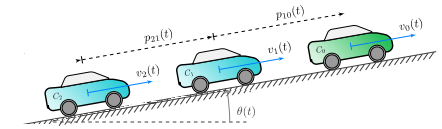
\includegraphics[width=15cm]{Untitled.png}
	\caption{Schematic of 2 car cooperative cruise control system}
	\label{fig:cruise-2car-system}
\end{figure*}


\section{Centralized and Decentralized tracking MPC}\label{sec:2}
Let ($A_i, B_i, C_i)$ be the minimal state realization of ($u_i, y_i$) input-output pair \cite{Ding2012} represented by the following model, for each player $i = 1,2$:
\begin{itemize}
    \item Model for Player 1:\newline$x_1^+ = A_1x_1 + B_1_1u_1 + B_1_2u_2, x_1(0) = x_1_0$
\newline $y_1 = C_1x_1$
    \item Model for Player 2:\newline$x_2^+ = A_2x_2 + B_2_2u_2 + B_2_1u_1, x_2(0) = x_2_0$
\newline $y_2 = C_2x_2$
\end{itemize}
\newline
Defining the cost for player 1:
$J_1(x_1(0),u_1,u_2) = p(y_1(N)-\overline{y}_1(N)) + \sum_{k=0}^{N-1} q(y_1(N)-\overline{y}_1(N),u_1(k))$

The cost of player 2 is defined analogously.

\begin{enumerate}[2.1]
	\item \textbf{Centralized Tracking MPC}-
    As we have seen above, the objective of each player is affected by the other player's input. In centralized control, the two players share the same objective\cite{Ding2012}, so the new cost function for the centralized problem can be given by:\newline
    $J(x_1,x_2,u_1,u_2)=\rho J_1(x_1,u_1,u_2)+\rho J_2(x_2,u_2,u_1)$ such that $x_i^+=A_ix_i+B_iu_i$, $y_i=C_ix_i$, for each player $i=1,2$
    being $\rho_1$ and $\rho_2$ the weights of the two players in the cost function and the $Q,R,P$ matrices defined by:
    $Q=$
    \begin{bmatrix}
    \rho _1Q_1 & 0\\
     0 & \rho _2Q_2
    \end{bmatrix}, 
    $R=$
    \begin{bmatrix}
    \rho _1R_1 & 0\\
     0 & \rho _2R_2
    \end{bmatrix}, 
    $P=$
    \begin{bmatrix}
    \rho _1P_1 & 0\\
     0 & \rho _2P_2
    \end{bmatrix}.
    \newline The equivalent batch formulation is \newline 
    %  \[\min_{U}\]
    $\underset{U}{min}\quad J=U^T\tilde{R}U+2U^T\tilde{S}(\overline{F}x(0)-\overline{Y})+
    (\overline{F}x(0)-\overline{Y})^T\overline{Q}(\overline{F}x(0)-\overline{Y})$
    \newline and the optimal control sequence is $U^*=K^*x(0) + K^*_y\overline{Y}=\{u^*(0),u^*(1),...,u^*(N-1)\}$
    with \newline$K^*=-K^*_y\overline{F}$ and $K^*_y=\tilde{R}^{-1}\tilde{S}$
    
	\item \textbf{Decentralized Tracking MPC}- On the other hand, decentralized MPC optimized only the local objectives and has no information about the actions of other subsystems \cite{Ding2012}. For each player $i$, the tracking MPC problem is \cite{Guerreiro2021}:\newline
	$\underset{min}{U_i}\quad J_i(x_i(0),U_i)=p(y_i(N)-\overline{y}_i(N)) + \sum_{k=0}^{N-1} q(y_i(N)-\overline{y}_i(N),u_i(k))$, such that $x_i^+=A_ix_i+B_{ii}$ and $y_i=C_ix_i$. \newline
	The equivalent batch formulation for player $i$ is  $\underset{U_i}{min}\quad J_i=U_i^T\tilde{R_i}U_i+2U_i^T\tilde{S_i}(\overline{F_i}x(0)-\overline{Y})+
    (\overline{F_i}x(0)-\overline{Y})^T\overline{Q_i}(\overline{F_i}x(0)-\overline{Y})$\newline 
    and the optimal control sequence is $U_i^*=K_i^*x_i(0) + K^*_{yi}\overline{Y_i}=\{u_i^*(0),u_i^*(1),...,u_i^*(N-1)\}$
	
\end{enumerate}

\section{Two-Follower Problem}\label{sec:mpc-design-unc}

In this section, we will design the adaptive cruise model-based predictive controller, considering embedded integral action the limitations of the system.

\begin{enumerate}[3.1]
	\item Considering the modelling previously developed in Project 1 for one generic, non-linearized follower vehicle:
	$\bvec{\Dot{x}_i}(t)=\blkmat{\Dot{{p_j_i}}(t) \\ \Dot{v}_i(t)}=    
	\begin{bmatrix}
    v_j(t) - v_i(t)\\
    \frac{F_i(t)}{m} - \frac{1}{2m}\rho A C_d (v_i(t) + w(t))^2 - g\sin{\theta(t)}
    \end{bmatrix}$
    
    To avoid measurement, model errors and external perturbations that affect performance, the developed controller features an integral effect. For this, an incremental state vector is defined:
    $\bvec{x}(k)=\blkmat{\Delta x_d(k)^T & y_d(k)^T}^T$
    and the respective extended model is: 
    $A=$\begin{bmatrix}
    A_d & 0 \\
    C_dA_c & I
    \end{bmatrix}, 
    $B=$\begin{bmatrix}
        B_d \\
        C_dB_d
    \end{bmatrix} and
    $C=$\begin{bmatrix}
        0 & I
    \end{bmatrix}
    
    
    By consequence, the calculated control action is given in terms of $\Delta u$, therefore the control action is then changed to:
    $\bvec{u}(k)= \Delta u(k) + u(k-1)$
    
\end{enumerate}

\begin{enumerate}[3.2]

    \item \textbf{Centralized Two-Follower Problem}- For the centralized approach both vehicles dynamics must be incorporated in one  state-space representation, as defined in ~\ref{sec:2}. After linearization and neglecting the disturbances, the centralized model is given by: 
    
    $\bvec{\Dot{x}}(t)=\blkmat{p_1_0(t) \\ v_1(t) \\ p_2_1(t) \\ v_2(t)}=    
	\begin{bmatrix}
    0 & -1 & 0 & 0\\
    0 &-\frac{\rho A C_d v_e}{m} & 0 & 0\\
    0 & 1 & 0 & -1\\
    0 & 0 & 0 & -\frac{\rho A C_d v_e}{m}
    \end{bmatrix}
    \blkmat{p_1_0(t) \\ v_1(t) \\ p_2_1(t) \\ v_2(t)}+
    \begin{bmatrix}
    0 & 0\\
    \frac{1}{m} & 0\\
    0 & 0\\
    0 & \frac{1}{m}
    \end{bmatrix}
    \begin{bmatrix}
    u_1(k)\\
    u_2(k)
    \end{bmatrix}$
    \newline
    $\bvec{y}(k)=
    \begin{bmatrix}
    1 & 0 & 0 & 0\\
    0 & 0 & 1 & 0
    \end{bmatrix}
    \blkmat{p_1_0(t) \\ v_1(t) \\ p_2_1(t) \\ v_2(t)}$
    
    The $\emph{1}$ value on the second column and third line of the state matrix establishes the communication between both players.
    Centralized control has full information on the vehicle's states, and the optimization problem is solved knowing all decision variables.\cite{Ding2012}\newline
    The for the batch approach for the equivalent unconstrained quadratic optimization problem are:

        $\overline{Q}=diag(Q_{n=0},...,Q_{n=N-1},P) $ \newline $\overline{R}=diag(R_{n=0},...,R_{n=N-1})\\H=diag(C_{n=0},...,C_{n=N-1})$\newline

    with $Q=diag(Q_1,Q_2)$ and $R=diag(r_1,R_2)$ \newline
    The final matrices are \newline
  
        $\tilde{R}=\overline{G}^T\overline{Q}\overline{G}+\overline{R}$ \newline
        $\tilde{S}=\overline{G}^T\overline{Q} $ \newline
        $\overline{F}=
                \begin{bmatrix}
                C \\
                CA \\
                CA^2 \\
                \vdots \\
                CA^{N-1}
                \end{bmatrix}$ \newline
        $\overline{G}=
              \begin{bmatrix}
              0   &  0  &  \dots  &  0 \\
              CB  &  0  &  \dots  &  0 \\
              \vdots  &  \vdots  & \vdots &\vdots \\
              CA^{N-1}B & CA^{N-2} & \dots & CB
              \end{bmatrix}$\newline
        $K_y=\overline{R}^{-1}\tilde{S}$\newline
        $K=\overline{R}^{-1}\tilde{S}\overline{F}$
  
    
    
\end{enumerate}

\begin{enumerate}[3.3]
    \item \textbf{Decentralized Two-Follower Problem}- As mentioned in \ref{sec:2}, the decentralized MPC does not incorporate in each player the information of other players, and their objectives are set independently. Therefore, the decentralized model will be given by:
    $\bvec{\Dot{x}}(t)=\blkmat{p_1_0(t) \\ v_1(t) \\ p_2_1(t) \\ v_2(t)}=    
	\begin{bmatrix}
    0 & -1 & 0 & 0\\
    0 &-\frac{\rho A C_d v_e}{m} & 0 & 0\\
    0 & 0 & 0 & -1\\
    0 & 0 & 0 & -\frac{\rho A C_d v_e}{m}
    \end{bmatrix}
    \blkmat{p_1_0(t) \\ v_1(t) \\ p_2_1(t) \\ v_2(t)}+
    \begin{bmatrix}
    0 & 0\\
    \frac{1}{m} & 0\\
    0 & 0\\
    0 & \frac{1}{m}
    \end{bmatrix}
    \begin{bmatrix}
    u_1(k)\\
    u_2(k)
    \end{bmatrix}$
    \newline
    $\bvec{y}(k)=
    \begin{bmatrix}
    1 & 0 & 0 & 0\\
    0 & 0 & 1 & 0
    \end{bmatrix}
    \blkmat{p_1_0(t) \\ v_1(t) \\ p_2_1(t) \\ v_2(t)}$\newline
    As we have just noticed, the previous member of the centralized model that established the communication between players is now set to zero.\newline
    The batch matrices are calculated in the same way as we calculated for centralized MPC, but instead of using $Q=diag(Q_1,Q_2)$ and $R=diag(r_1,R_2)$, we use the cost matrices $Q_1, Q_2, R_1, R_2$ to calculate the batch matrices for each player.
    
\end{enumerate}

\section{Simulations}\label{sec:sim}

The developed centralized and decentralized controllers were simulated in MATLAB, utilizing the following controller parameters:
$ N = 20, 
P_i = 1, 
Q_i = 10000, 
R_i = 0.001, 
$

 \begin{figure}[!ht]
 	\centering
 	%\resizebox{0.9\linewidth}{!}{\input{problem.png}}
 	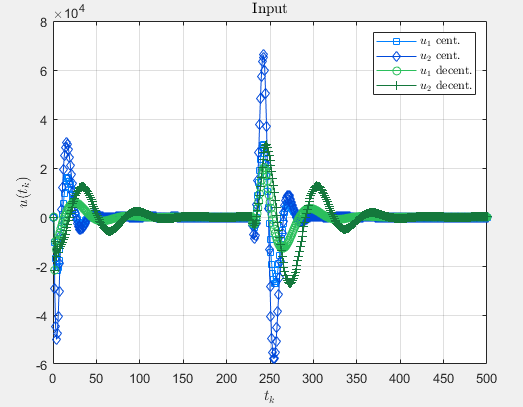
\includegraphics[width=7cm]{cen_dec_unc_in.png}
 	\caption{Control action for the two car cooperative cruise control system}
 	\label{fig:control action}
 \end{figure}
 
 \begin{figure}[!ht]
 	\centering
 	%\resizebox{0.9\linewidth}{!}{\input{problem.png}}
 	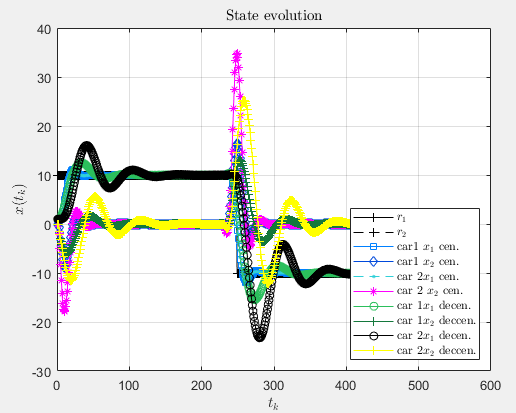
\includegraphics[width=7cm]{cen_dec_unc_out.png}
 	\caption{State evolution of the two car cooperative cruise control system}
 	\label{fig:output}
 \end{figure}
 
\vspace{6cm}

 \begin{figure}[!h]
 	\centering
 	%\resizebox{0.9\linewidth}{!}{\input{problem.png}}
 	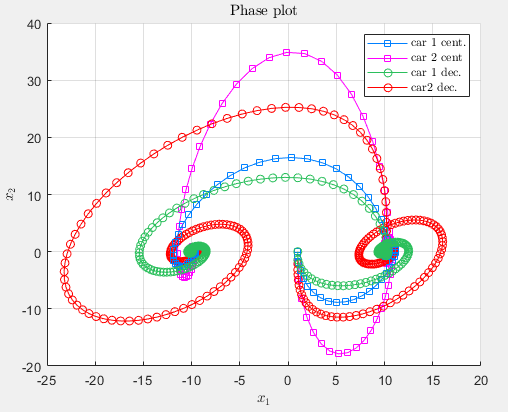
\includegraphics[width=7cm]{cen_dec_unc_states.png}
 	\caption{Phase plot of the two car cooperative cruise control system}
 	\label{fig:states}
 \end{figure}

Using the same parameters, we now add some Gaussian noise to the system output.
 \begin{figure}[!ht]
 	\centering
 	%\resizebox{0.9\linewidth}{!}{\input{problem.png}}
 	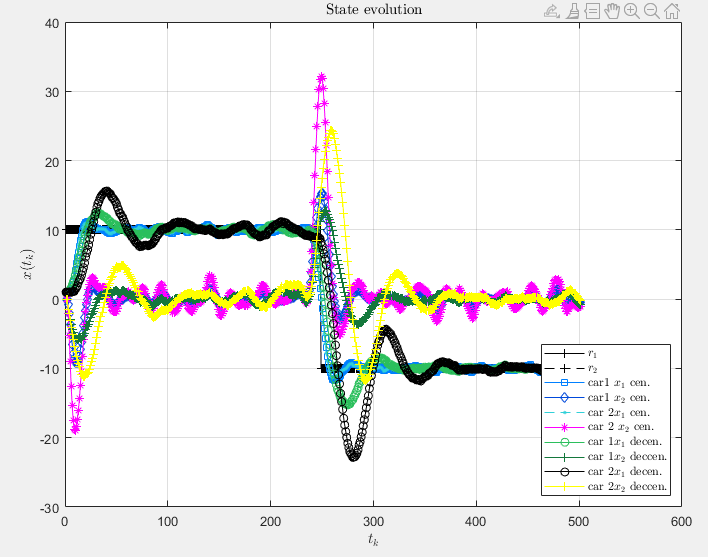
\includegraphics[width=7cm]{cen_dec_unc_out_noise.png}
 	\caption{State evolution of the two car cooperative cruise control system}
 	\label{fig:output_noise}
 \end{figure}
\section{Concluding remarks}

The centralized controller produces more abrupt control actions for each vehicle, that quickly stabilize as the reference is reached. As the controllers are completely unconstrained input wise, this effect doesn't present any problem or stress in the actuator, however this might be a problem in a practical implementation. In comparison, the decentralized controller's control action is smoother, but slightly oscillatory.

As for the state evolution, the decentralized controller has a slower response time and takes longer to settle to the reference, but nonetheless both controllers produce satisfactory results, neglecting the constraints that come with the car. The centralized controller appears to be a better solution for this specific two-vehicle problem, however in a real practical application a centralized system needs to have access to every known state and the computing capability of solving a generally more complex optimization problem.
When we added Gaussian noise, we see that the output produced by the decentralized model, is severally degraded when compared to the centralized. 
Concluding, decentralized control as some implementation advantage, due to its simplicity, but the resulting performance may be quite poor. \cite{Ding2012}
% The developed controllers provide us with a good basis to develop a distributed MPC controller, and to expand from two-follower cooperative cruise control into a multiple-vehicle platooning approach.

\nocite{*}
\bibliographystyle{plain}
%\bibliography{CPCS_P1_biblios}
\bibliography{Lab2}
	
\end{document}

